
\documentclass[UTF8,12pt,a4paper]{ctexart}
\usepackage{amsmath,amssymb,graphicx,geometry,float}
\geometry{left=2.5cm,right=2.5cm,top=2.5cm,bottom=2.5cm}

\title{小车倒立摆控制器设计报告}
\author{姓名：\underline{\hspace{3cm}} \quad 学号：\underline{\hspace{3cm}}}
\date{\today}

\begin{document}
\maketitle

\section{项目背景}

小车倒立摆系统是控制理论中的经典对象，具有非线性、强耦合和开环不稳定等特点。
本次作业以小车倒立摆为对象，完成状态空间建模、状态反馈控制、LQR 调节器设计以及
类 \texttt{systune} 的自动调参仿真。

\section{状态空间模型}

选取系统状态变量为
\[
X=
\begin{bmatrix}
x & \dot{x} & \theta & \dot{\theta}
\end{bmatrix}^T,
\]
其中 $x$ 表示小车位移，$\theta$ 表示摆杆偏离竖直方向的角度。

线性化后的状态空间模型为
\[
\dot{X} = AX + Bu.
\]

在本仿真中，系统参数取
\[
M=0.5,\quad m=0.2,\quad b=0.1,\quad l=0.3,\quad g=9.81.
\]

对应的系统矩阵为
\[
A=
\begin{bmatrix}
0 & 1 & 0 & 0\\
0 & -b/M & -mg/M & 0\\
0 & 0 & 0 & 1\\
0 & -b/(Ml) & (M+m)g/(Ml) & 0
\end{bmatrix},
\quad
B=
\begin{bmatrix}
0\\
1/M\\
0\\
-1/(Ml)
\end{bmatrix}.
\]

\section{LQR 状态反馈控制}

LQR 控制器采用状态反馈形式
\[
u=-KX.
\]

其性能指标为
\[
J=\int_0^\infty \left(X^TQX+u^TRu\right)\,dt.
\]

本实验中取
\[
Q=\mathrm{diag}(10,1,100,1),\quad R=0.01.
\]

计算得到的 LQR 状态反馈增益为：
\begin{verbatim}
K_lqr = [[ -31.6228  -26.7753 -144.2426  -20.326 ]]
\end{verbatim}

LQR 闭环极点为：
\begin{verbatim}
[-69.5513+0.j     -9.8558+0.j     -1.3745+1.062j  -1.3745-1.062j]
\end{verbatim}

\section{类 systune 的状态反馈自动调参}

MATLAB 中的 \texttt{systune} 可以根据给定调参目标自动整定控制器参数。
Python 中没有完全相同的函数，因此本文采用 \texttt{scipy.optimize} 构造类似调参过程。
调参变量仍然为状态反馈矩阵 $K$，控制律仍为
\[
u=-KX.
\]

调参目标包括：

\begin{itemize}
    \item 闭环极点实部小于 $-1$，保证系统具有足够衰减速度；
    \item 闭环极点阻尼比不小于 $0.6$，减少振荡；
    \item 闭环极点自然频率不超过 $30\,\mathrm{rad/s}$，避免控制输入过于激烈；
    \item 对过大的反馈增益加入惩罚项。
\end{itemize}

优化后得到的状态反馈增益为：
\begin{verbatim}
K_tuned = [[ -1.9635  -3.1061 -29.6516  -3.2398]]
\end{verbatim}

类 systune 调参后的闭环极点为：
\begin{verbatim}
[-6.7935+9.0712j -6.7935-9.0712j -0.9999+0.j     -0.9999-0.j    ]
\end{verbatim}

优化目标函数值为：
\begin{verbatim}
0.0903868
\end{verbatim}

\section{仿真结果}

初始状态设置为
\[
X(0)=
\begin{bmatrix}
0.1 & 0 & 0.1 & 0
\end{bmatrix}^T.
\]

\begin{figure}[H]
\centering
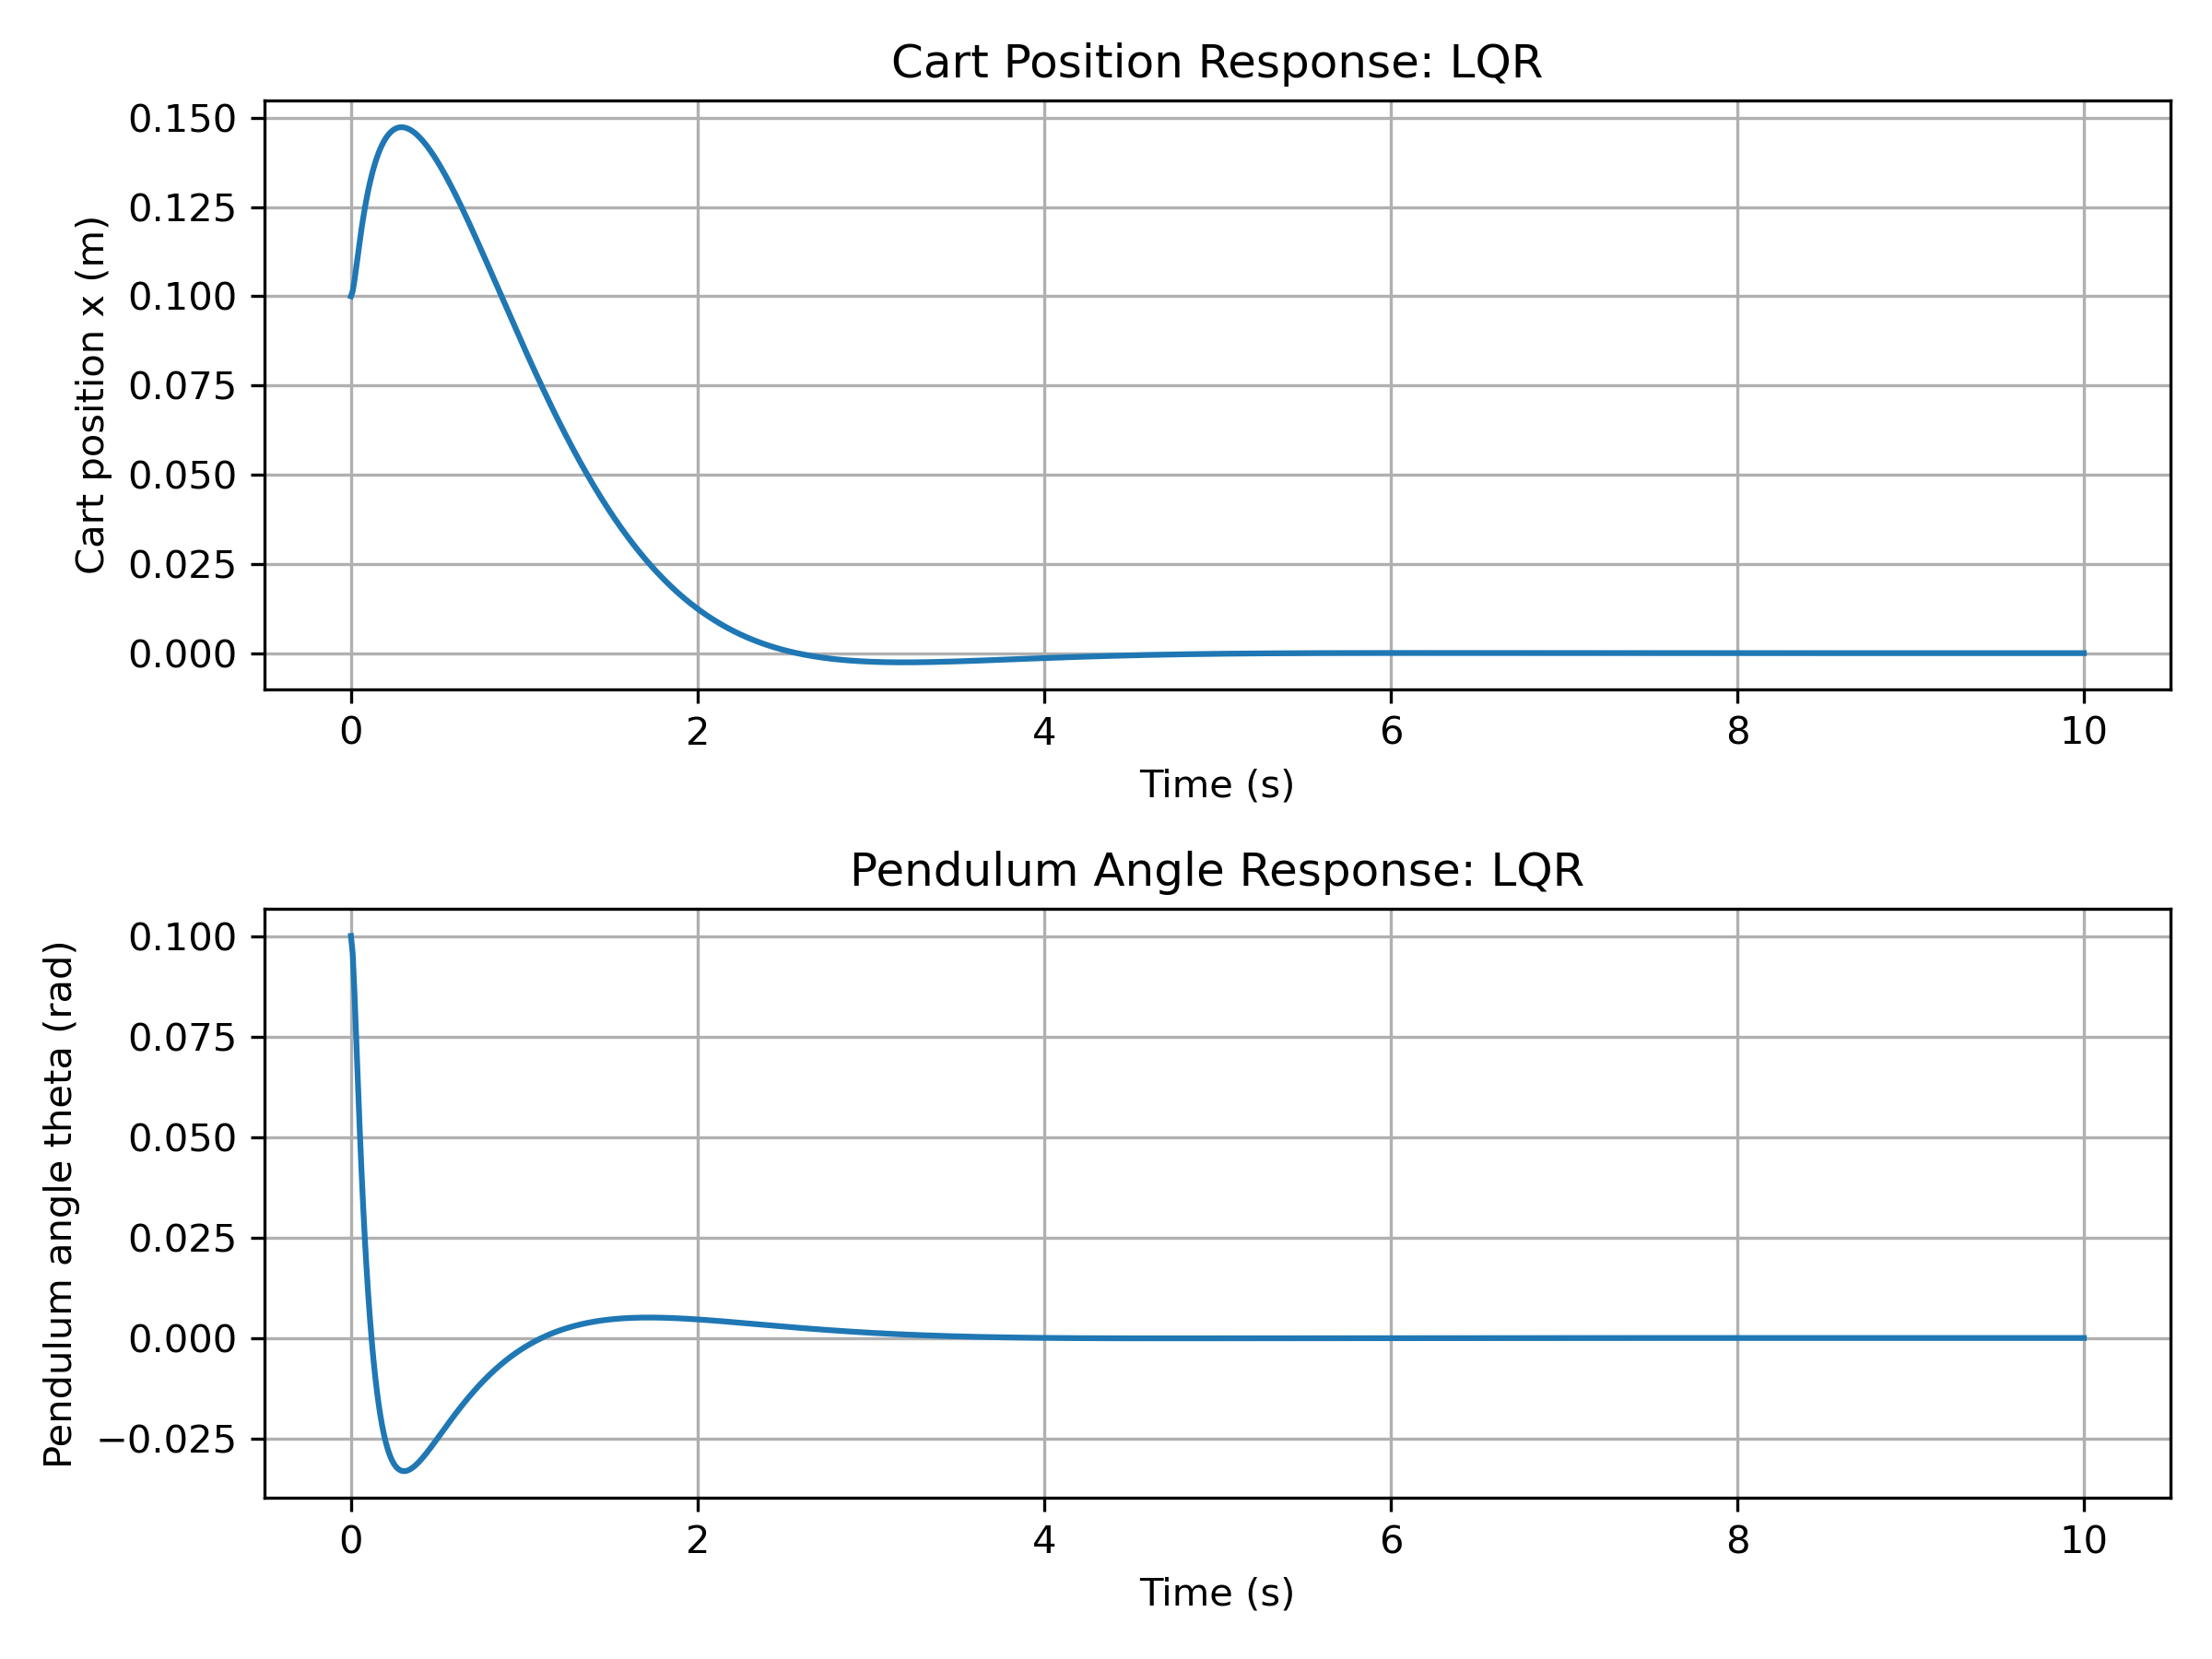
\includegraphics[width=0.85\textwidth]{pendulum_lqr_response.png}
\caption{LQR 控制下的小车位移和摆杆角度响应}
\end{figure}

\begin{figure}[H]
\centering
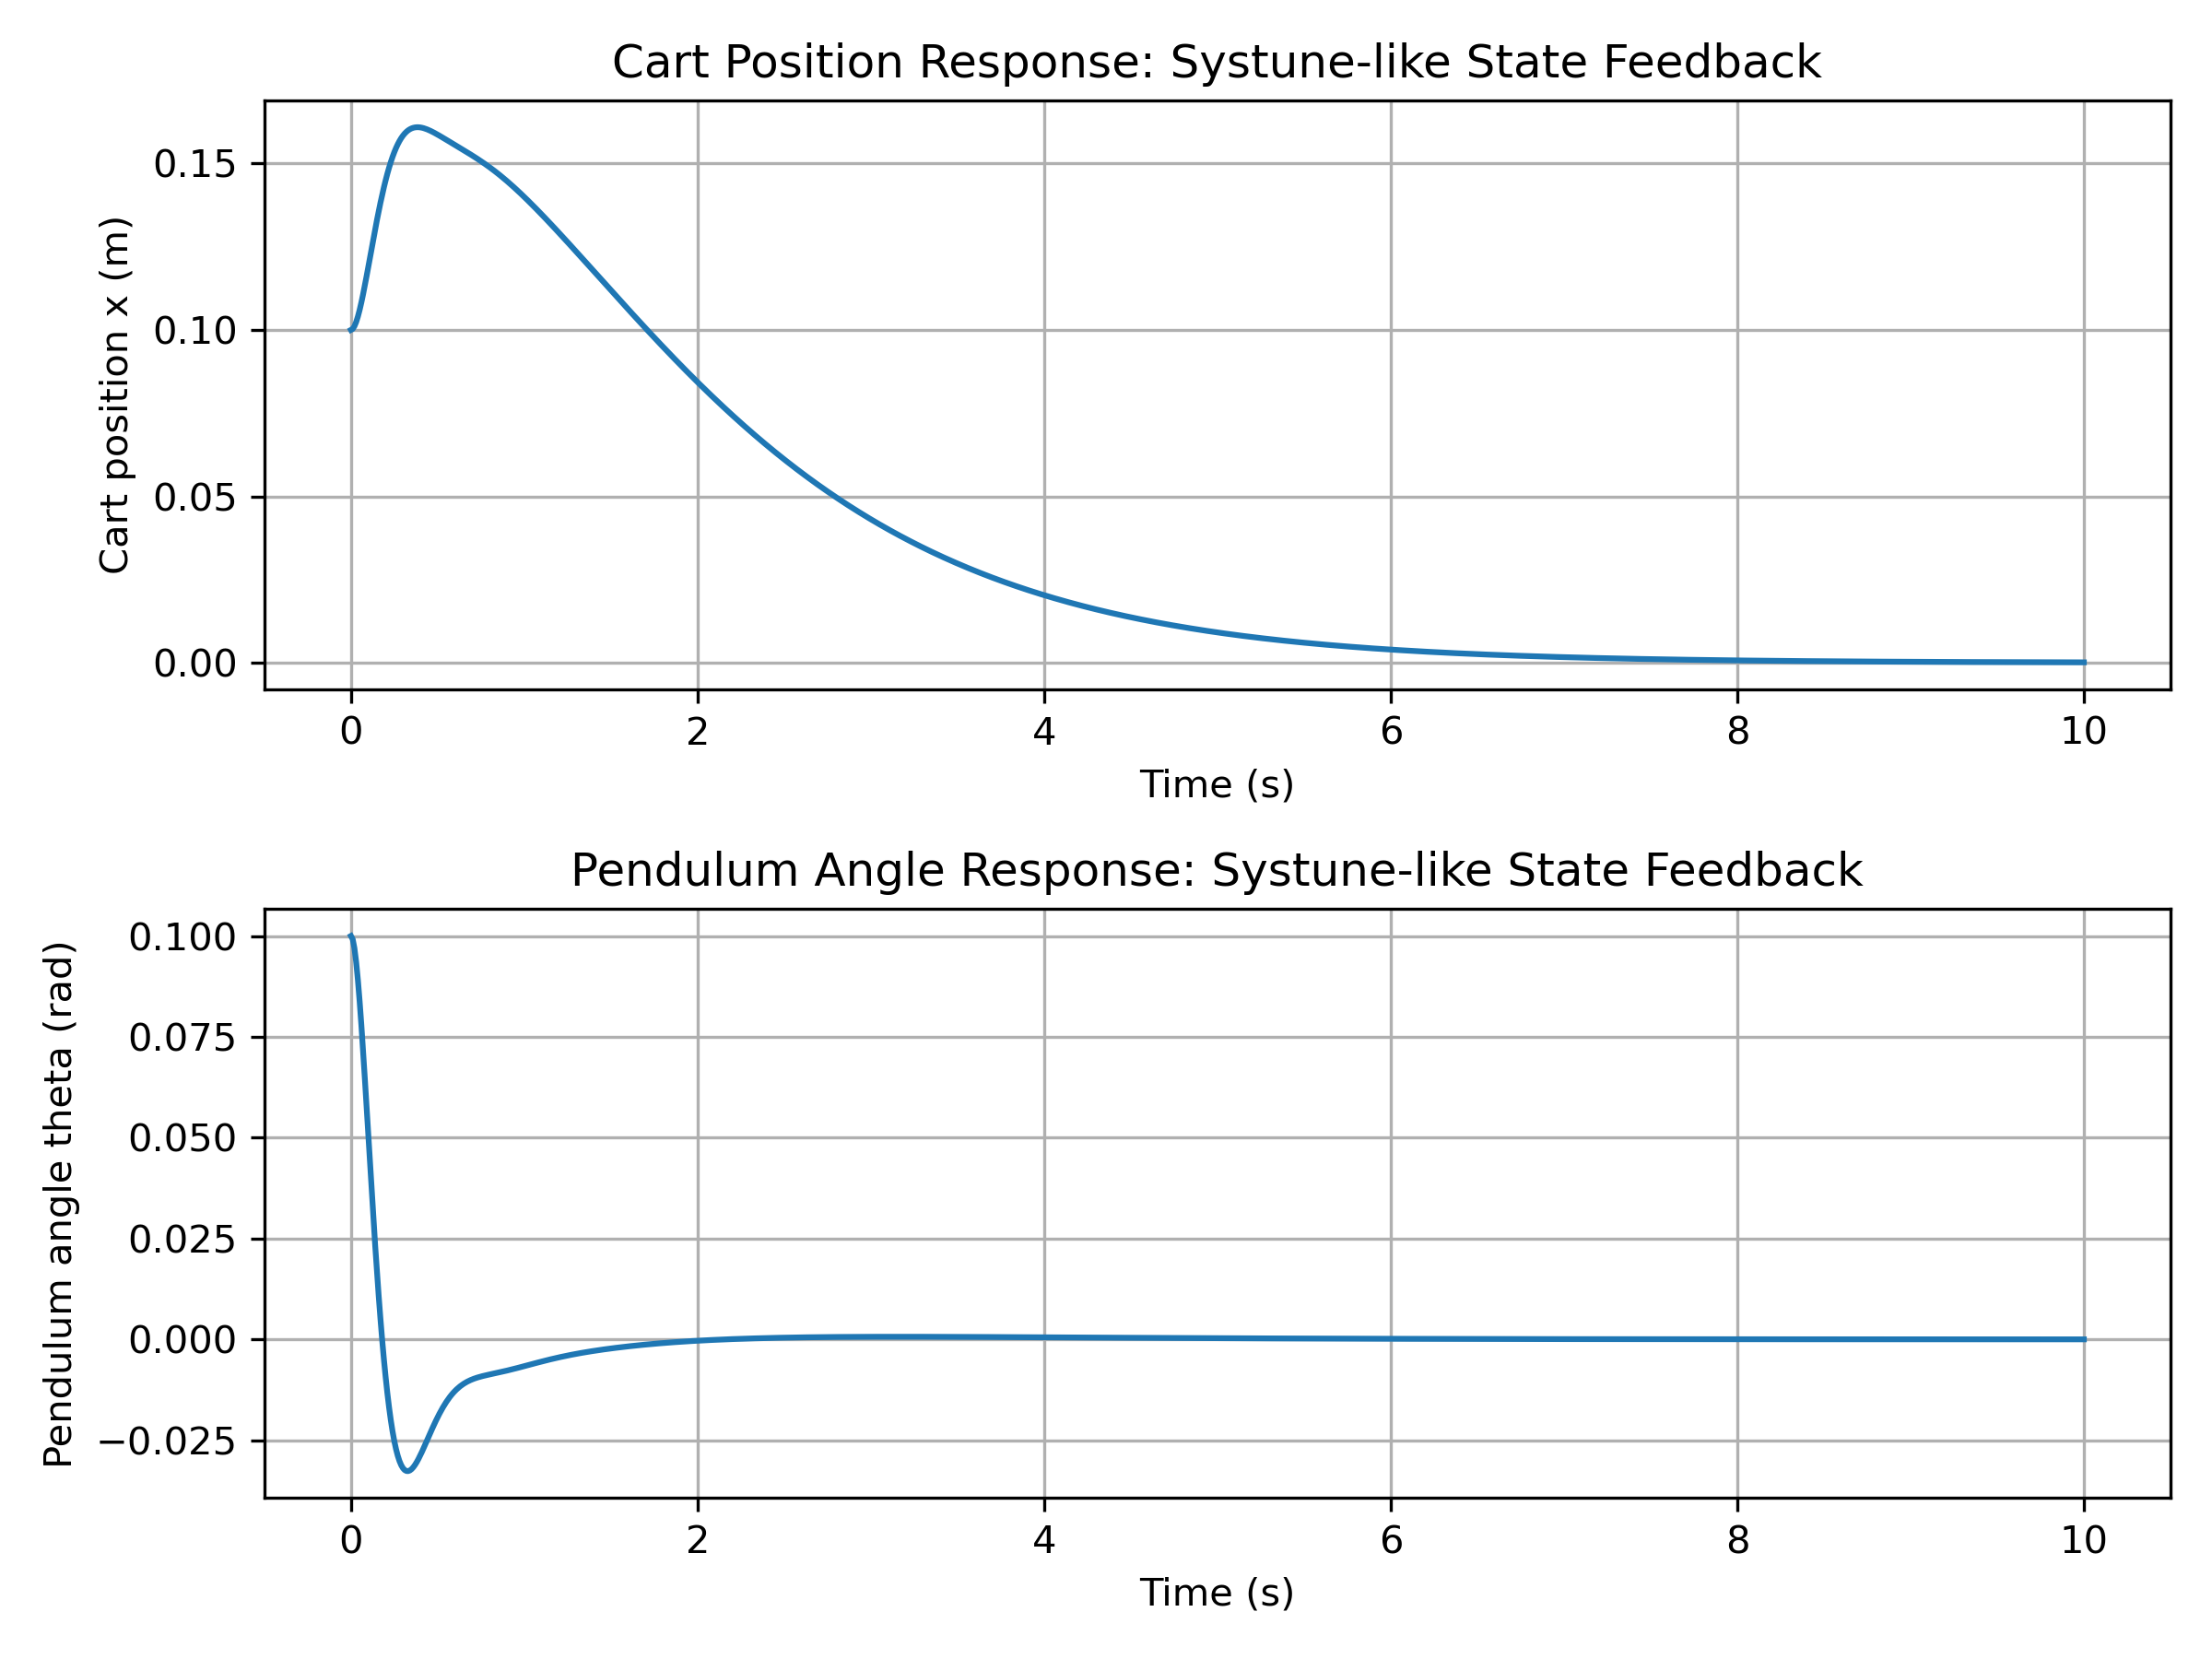
\includegraphics[width=0.85\textwidth]{pendulum_systune_like_response.png}
\caption{类 systune 状态反馈控制下的小车位移和摆杆角度响应}
\end{figure}

\begin{figure}[H]
\centering
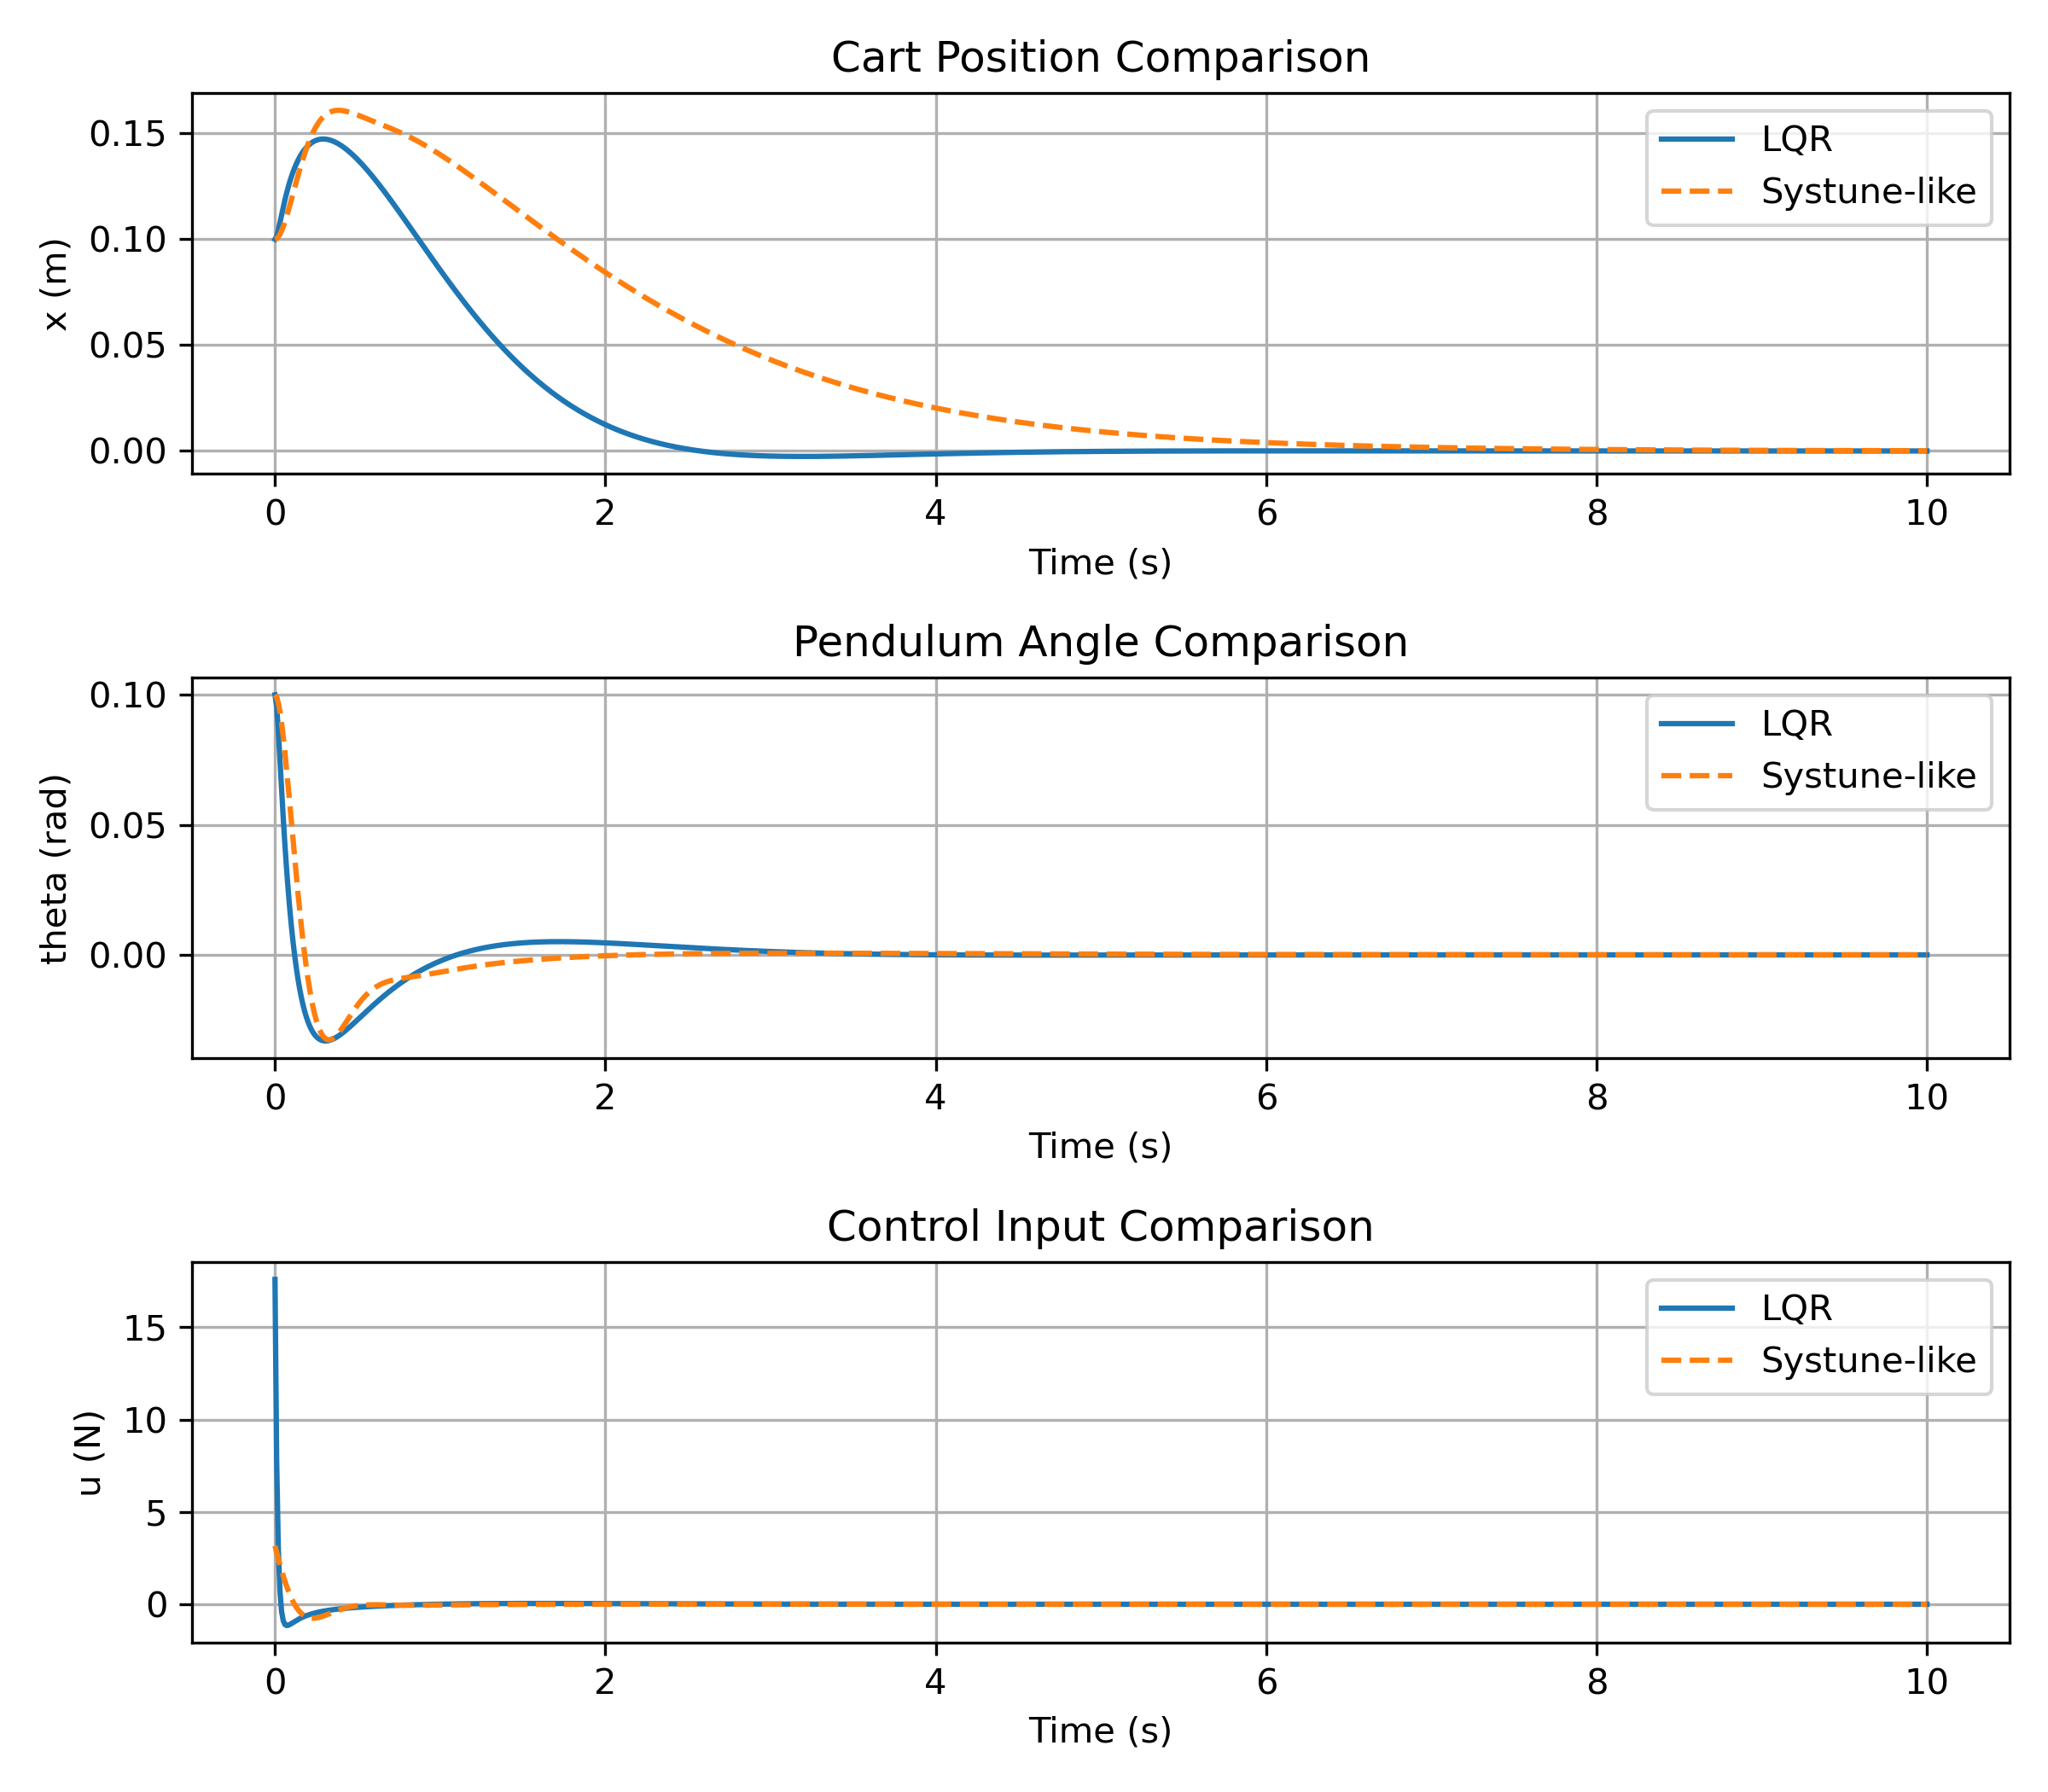
\includegraphics[width=0.85\textwidth]{pendulum_lqr_vs_systune_like.png}
\caption{LQR 与类 systune 状态反馈控制效果对比}
\end{figure}

\section{结果分析}

从仿真结果可以看出，LQR 控制器能够使小车倒立摆系统从初始偏差状态逐渐回到平衡位置。
摆杆角度 $\theta$ 逐渐收敛到零，说明倒立摆被稳定在竖直平衡位置附近。

类 \texttt{systune} 方法则通过极点约束自动调整反馈矩阵。
与 LQR 方法相比，该方法更接近工程调参思路：先给出期望的闭环稳定性、阻尼比和频率范围，
再由优化算法寻找满足要求的反馈增益。

需要注意的是，本文的 Python 实现并不是 MATLAB \texttt{systune} 的完全替代，
而是根据相同思想实现的状态反馈自动调参方法。

\section{总结}

本次作业完成了小车倒立摆系统的状态空间建模、LQR 状态反馈控制器设计、
类 \texttt{systune} 状态反馈自动调参以及仿真绘图。通过本实验可以看出，
对于小车倒立摆这类开环不稳定系统，状态反馈控制能够有效利用系统全部状态信息，
实现闭环稳定控制。LQR 方法具有明确的最优控制理论基础，而类 \texttt{systune} 方法
则体现了基于工程指标的自动调参思想。

\end{document}
